
%(BEGIN_QUESTION)
% Copyright 2014, Tony R. Kuphaldt, released under the Creative Commons Attribution License (v 1.0)
% This means you may do almost anything with this work of mine, so long as you give me proper credit

Solve for all voltages and currents in this series RC circuit:

$$\includegraphics[width=15.5cm]{i01052x01.eps}$$

\underbar{file i01052}
%(END_QUESTION)





%(BEGIN_ANSWER)

$V_C = 14.39 \hbox{ volts RMS}$

\vskip 10pt

$V_R = 4.248 \hbox{ volts RMS}$

\vskip 10pt

$I = 903.9 \> \mu \hbox{A RMS}$

%(END_ANSWER)





%(BEGIN_NOTES)

Nothing special here -- just a straightforward exercise in series AC circuit calculations.

\vskip 10pt

Students often have difficulty formulating a method of solution: determining what steps to take to get from the given conditions to a final answer.  While it is helpful at first for you (the instructor) to show them, it is bad for you to show them too often, lest they stop thinking for themselves and merely follow your lead.  A teaching technique I have found very helpful is to have students come up to the board (alone or in teams) in front of class to write their problem-solving strategies for all the others to see.  They don't have to actually do the math, but rather outline the steps they would take, in the order they would take them.  The following is a sample of a written problem-solving strategy for analyzing a series resistive-reactive AC circuit:

\vskip 10pt

\goodbreak

{\bf Step 1:} Calculate all reactances ($X$).

{\bf Step 2:} Draw an impedance triangle ($Z$ ; $R$ ; $X$), solving for $Z$

{\bf Step 3:} Calculate circuit current using Ohm's Law: $I = {V \over Z}$

{\bf Step 4:} Calculate series voltage drops using Ohm's Law: $V = {I Z}$

{\bf Step 5:} Check work by drawing a voltage triangle ($V_{total}$ ; $V_1$ ; $V_2$), solving for $V_{total}$

\vskip 10pt

By having students outline their problem-solving strategies, everyone gets an opportunity to see multiple methods of solution, and you (the instructor) get to see how (and if!) your students are thinking.  An especially good point to emphasize in these ``open thinking'' activities is how to check your work to see if any mistakes were made.

%INDEX% Electronics review: AC reactance and impedance

%(END_NOTES)


